%======================================================
% Technische Universitaet Darmstadt
% Fachbereich Elektrotechnik und Informationstechnik
% Fachbereich Informatik (Zweitmitglied)
% Fachgebiet Multimedia Kommunikation (KOM)
% Prof. Dr.-Ing. Ralf Steinmetz
%======================================================
% Template for Theses
% VERSION 1.0 (October 2009)
% Use pdfLaTeX (other possible, but not supported)
% Contact at KOM: Andr\'e Miede (andre.miede@kom...)
%======================================================
% Official TUD-LaTeX-files have to be installed:
% http://exp1.fkp.physik.tu-darmstadt.de/tuddesign/
% Refer to the manuals and forum for details
%======================================================
\documentclass[longdoc,accentcolor=tud9b,11pt,paper=a4,ngerman]{tudreport}
%======================================================
% colorback = Bereich unter Titel mit Hintergrundfarbe
% colorbacktitle = Titel mit Hintergrundfarbe (Akzent)
% KOM-Blau = accentcolor=tud1b		
% Grau = accentcolor=tud0a 
% blackrule fuer schwarze Leiste
% nochapterpage = do not start chapters on new page
% oneside = print only on one side of the page
%======================================================

%======================================================
% General package loading and definitions
%======================================================
\usepackage{inputenc}
\usepackage{textcomp} 
\usepackage{ngerman}
\usepackage[american,ngerman]{babel}
\usepackage{xspace}
\usepackage{placeins}
\usepackage[fleqn]{amsmath} % math environments and more by the AMS 
\newcounter{dummy} % necessary for correct hyperlinks (to index, bib, etc.)
\newcommand{\myfloatalign}{\centering} % how all the floats will be aligned

%======================================================
% KOM-modifications of the TUD-layout
%======================================================
% reduce font size of page footers and headers (fancyhdr)
\renewcommand{\footerfont}{\fontfamily{\sfdefault}\fontseries{m}\fontshape{n}\footnotesize\selectfont}
% remove space between items 
\usepackage{enumitem}
	\setenumerate{noitemsep}
	\setitemize{noitemsep}
	\setdescription{noitemsep}
%\setlist{nolistsep}

%======================================================
% Package loading for example contents (content.tex)
%======================================================
\usepackage{tabularx} % better tables
\setlength{\extrarowheight}{3pt} % increase table row height
\usepackage{booktabs,lipsum}
\usepackage{color}
\usepackage{colortbl}
\usepackage{caption}
\captionsetup{format=hang,font=small}
\usepackage[square,numbers]{natbib}
\usepackage{subfig}
\usepackage[stable,bottom]{footmisc}
\usepackage{listings}
\definecolor{dunkelgrau}{rgb}{0.8,0.8,0.8}
\usepackage{pdfpages}
%======================================================
% Important information: to be set here and only here
%======================================================
\newcommand{\komTitle}{Capturing Reality\xspace}
\newcommand{\komThesisType}{Projektbericht\xspace} % Diplomarbeit Studienarbeit Master-Arbeit Bachelor-Arbeit
\newcommand{\komID}{}
\newcommand{\komName}{Yannick Drost, Florian Herrmann, Pascal Schardt\xspace}
\newcommand{\komSubmissionDate}{31. M\"arz 2015\xspace}% use only this date format
\newcommand{\komGutachter}{Gutachter: Dr.-Ing. Michael Goesele\xspace}
\newcommand{\komBetreuer}{Betreuer: M.Sc. Simon Fuhrmann\xspace}

%======================================================
% Setup for hyperref
%======================================================
\usepackage[pdftex,hyperfootnotes=true,pdfpagelabels]{hyperref}
	\pdfcompresslevel=9
	\pdfadjustspacing=1 
\hypersetup{%
    colorlinks=false, linktocpage=false, pdfstartpage=1, pdfstartview=FitV,%
    breaklinks=true, pdfpagemode=UseNone, pageanchor=true, pdfpagemode=UseOutlines,%
    plainpages=false, bookmarksnumbered, bookmarksopen=true, bookmarksopenlevel=1,%
    hypertexnames=true, pdfhighlight=/O, %nesting=true,%frenchlinks,%
    %urlcolor=tud1b, linkcolor=tud1b, citecolor=tudtud1bccent,
    pdftitle={\komTitle, \komThesisType, \komID},%
    pdfauthor={\komName, KOM, TU Darmstadt},%
    pdfsubject={},%
    pdfkeywords={},%
    pdfcreator={},%
    pdfproducer={}%
}

%============================================
% Setup of the title page (do not change)
%============================================
\title{\komTitle}
\subtitle{\komThesisType}
\subsubtitle{\komName \\ \komID}
%\setinstitutionlogo[height]{kom_info}
\institution{\raggedleft 
	Fachbereich Informatik\\[\baselineskip]%
	Fachgebiet Graphisch-Interaktive Systeme \\%(KOM)
	Prof. Dr.-Ing. Michael Goesele%
}

%============================================
% Setup of the title backside (do not change)
%============================================
\lowertitleback{%
	Technische Universit\"at Darmstadt \\%
	Fachbereich Informatik\\[\baselineskip]%
	Fachgebiet Graphisch-Interaktive Systeme \\%(KOM)
	Prof. Dr.-Ing. Michael Goesele%
	%Department of Electrical Engineering and Information Technology \\%
	%Department of Computer Science (Adjunct Professor) \\[\baselineskip]%
	%Multimedia Communications Lab (KOM) \\%
	%Prof. Dr.-Ing. Ralf Steinmetz %
}

\uppertitleback{%
	\komTitle \\%
	\komThesisType \\%
	\komID \\[\baselineskip]%
	Eingereicht von \komName \\%
	Tag der Einreichung: \komSubmissionDate \\[\baselineskip]%
	\komGutachter \\%
	\komBetreuer \\%
	%\komExternerBetreuer%
}
	
%======================================================
% MAIN DOCUMENT STARTS HERE
%======================================================
\begin{document}
%======================================================
	% The front matter
	%======================================================
	\pagenumbering{roman}
	\frenchspacing
	\raggedbottom
	\selectlanguage{ngerman} % american ngerman
	\maketitle


%Chapterlabeling
%\titleformat{\chapter}
%  {\normalfont\LARGE\bfseries}{\thechapter}{1em}{\huge}
%\titlespacing*{\chapter}{0pt}{5.5ex plus 1ex minus .2ex}{2.3ex plus .2ex}
%Einkommentieren f\"ur gr\"o\ss ere \"Uberschriften

\setboolean{@twoside}{false} 


	\chapter*{Ehrenw\"ortliche Erkl\"arung}
	Hiermit versichere ich, den vorliegenden \komThesisType ohne Hilfe Dritter und nur mit den angegebenen Quellen 
    und Hilfsmitteln angefertigt zu haben. Alle Stellen, die aus den Quellen entnommen wurden, sind als solche 
    kenntlich gemacht worden. Diese Arbeit hat in dieser oder \"ahnlicher Form noch keiner Pr\"ufungsbeh\"orde vorgelegen.
	
	\vspace{1.5cm}
	\noindent Darmstadt, den \komSubmissionDate\hfill \komName

	\tableofcontents
	%\listoffigures
	%\listoftables
	\pagenumbering{arabic}
	%======================================================
	% The main matter (insert your contents here)
	%======================================================
	\cleardoublepage
	\chapter{Einf\"uhrung}
In Bezug auf die Steigerung der Rechenleistung von Computern werden auch die Anwendungsgebiete und Verfahren der Photogrammetrie\footnote{Auswerteverfahren zur Bestimmung der dreidimensionalen Form eines Objektes mittels Fotografien oder Messbildern.} immer leistungsf\"ahiger. Mittels Auswerteverfahren werden aus Fotografien eines Objektes die jeweils geometrische Beschaffenheit als auch Lage bestimmt. Die M\"oglichkeit reale Objekte zu digitalisieren erm\"oglicht eine interaktive Betrachtung der Modelle. \\
Eine Reihe an Fotografien des Frankfurter AfE-Turms kurz vor seiner Sprengung am 02.02.2014 soll f\"ur eine fehlerfreie grafische Rekonstruktion analysiert und aufbereitet werden. Die Herausforderung dieses Projektes zeigt sich anhand der gleichm\"a\ss igen Struktur und der sich wiederholenden Textur des zu untersuchenden Objektes. F\"ur eine Zuordnung einzelner Bildpaare werden, in beiden Bildern vorkommende gleiche Merkmale gesucht. Bereiche des einen Fotos werden jedoch, auf Grund der \"ahnlichkeit nichtzugeh\"origen Bildbereichen des anderen Fotos zugeteilt, weshalb eine Registrierung des Datensatzes fehlschl\"agt und letztlich kein verwendbares Ergebnis entsteht. 
Aufgabe ist eine qualitativ bessere Rekonstruktion des Frankfurter AfE-Turms. Um die Problematik mit der unzul\"anglichen Rekonstruktionsqualit\"at zu beheben, wird ein Ansatz zur Regionierung des Datensatzes implementiert um eine Voraussetzung f\"ur eine erfolgreiche Nachbildung zu liefern. Zu diesem Zweck werden die Bilder durch Abgrenzungen inhaltlich unterteilt, sodass  den anschlie\ss end extrahierten Bildmerkmalen zus\"atzliche Informationen zur relativen Lage zur Verf\"ugung stehen. Damit werden nur korrespondierende Bereiche innerhalb der Bilder f\"ur den Registrierungsansatz in Betracht gezogen. Die Fotos des Turms, welche hierf\"ur aus hinreichenden Winkeln akquiriert wurden, werden unter Ber\"ucksichtigung der Regionierung zueinander geometrisch erfasst. Durch diese entstehende Korrektur der Aufnahmepositionen einzelner Fotografien soll schlie\ss lich aus einer, zuvor undefinierbaren Punktwolke eine detailgetreue Nachbildung des Turms entstehen und ein qualitativ hochwertigeres Resultat erzielt werden.

\begin{figure}[h]
\centering
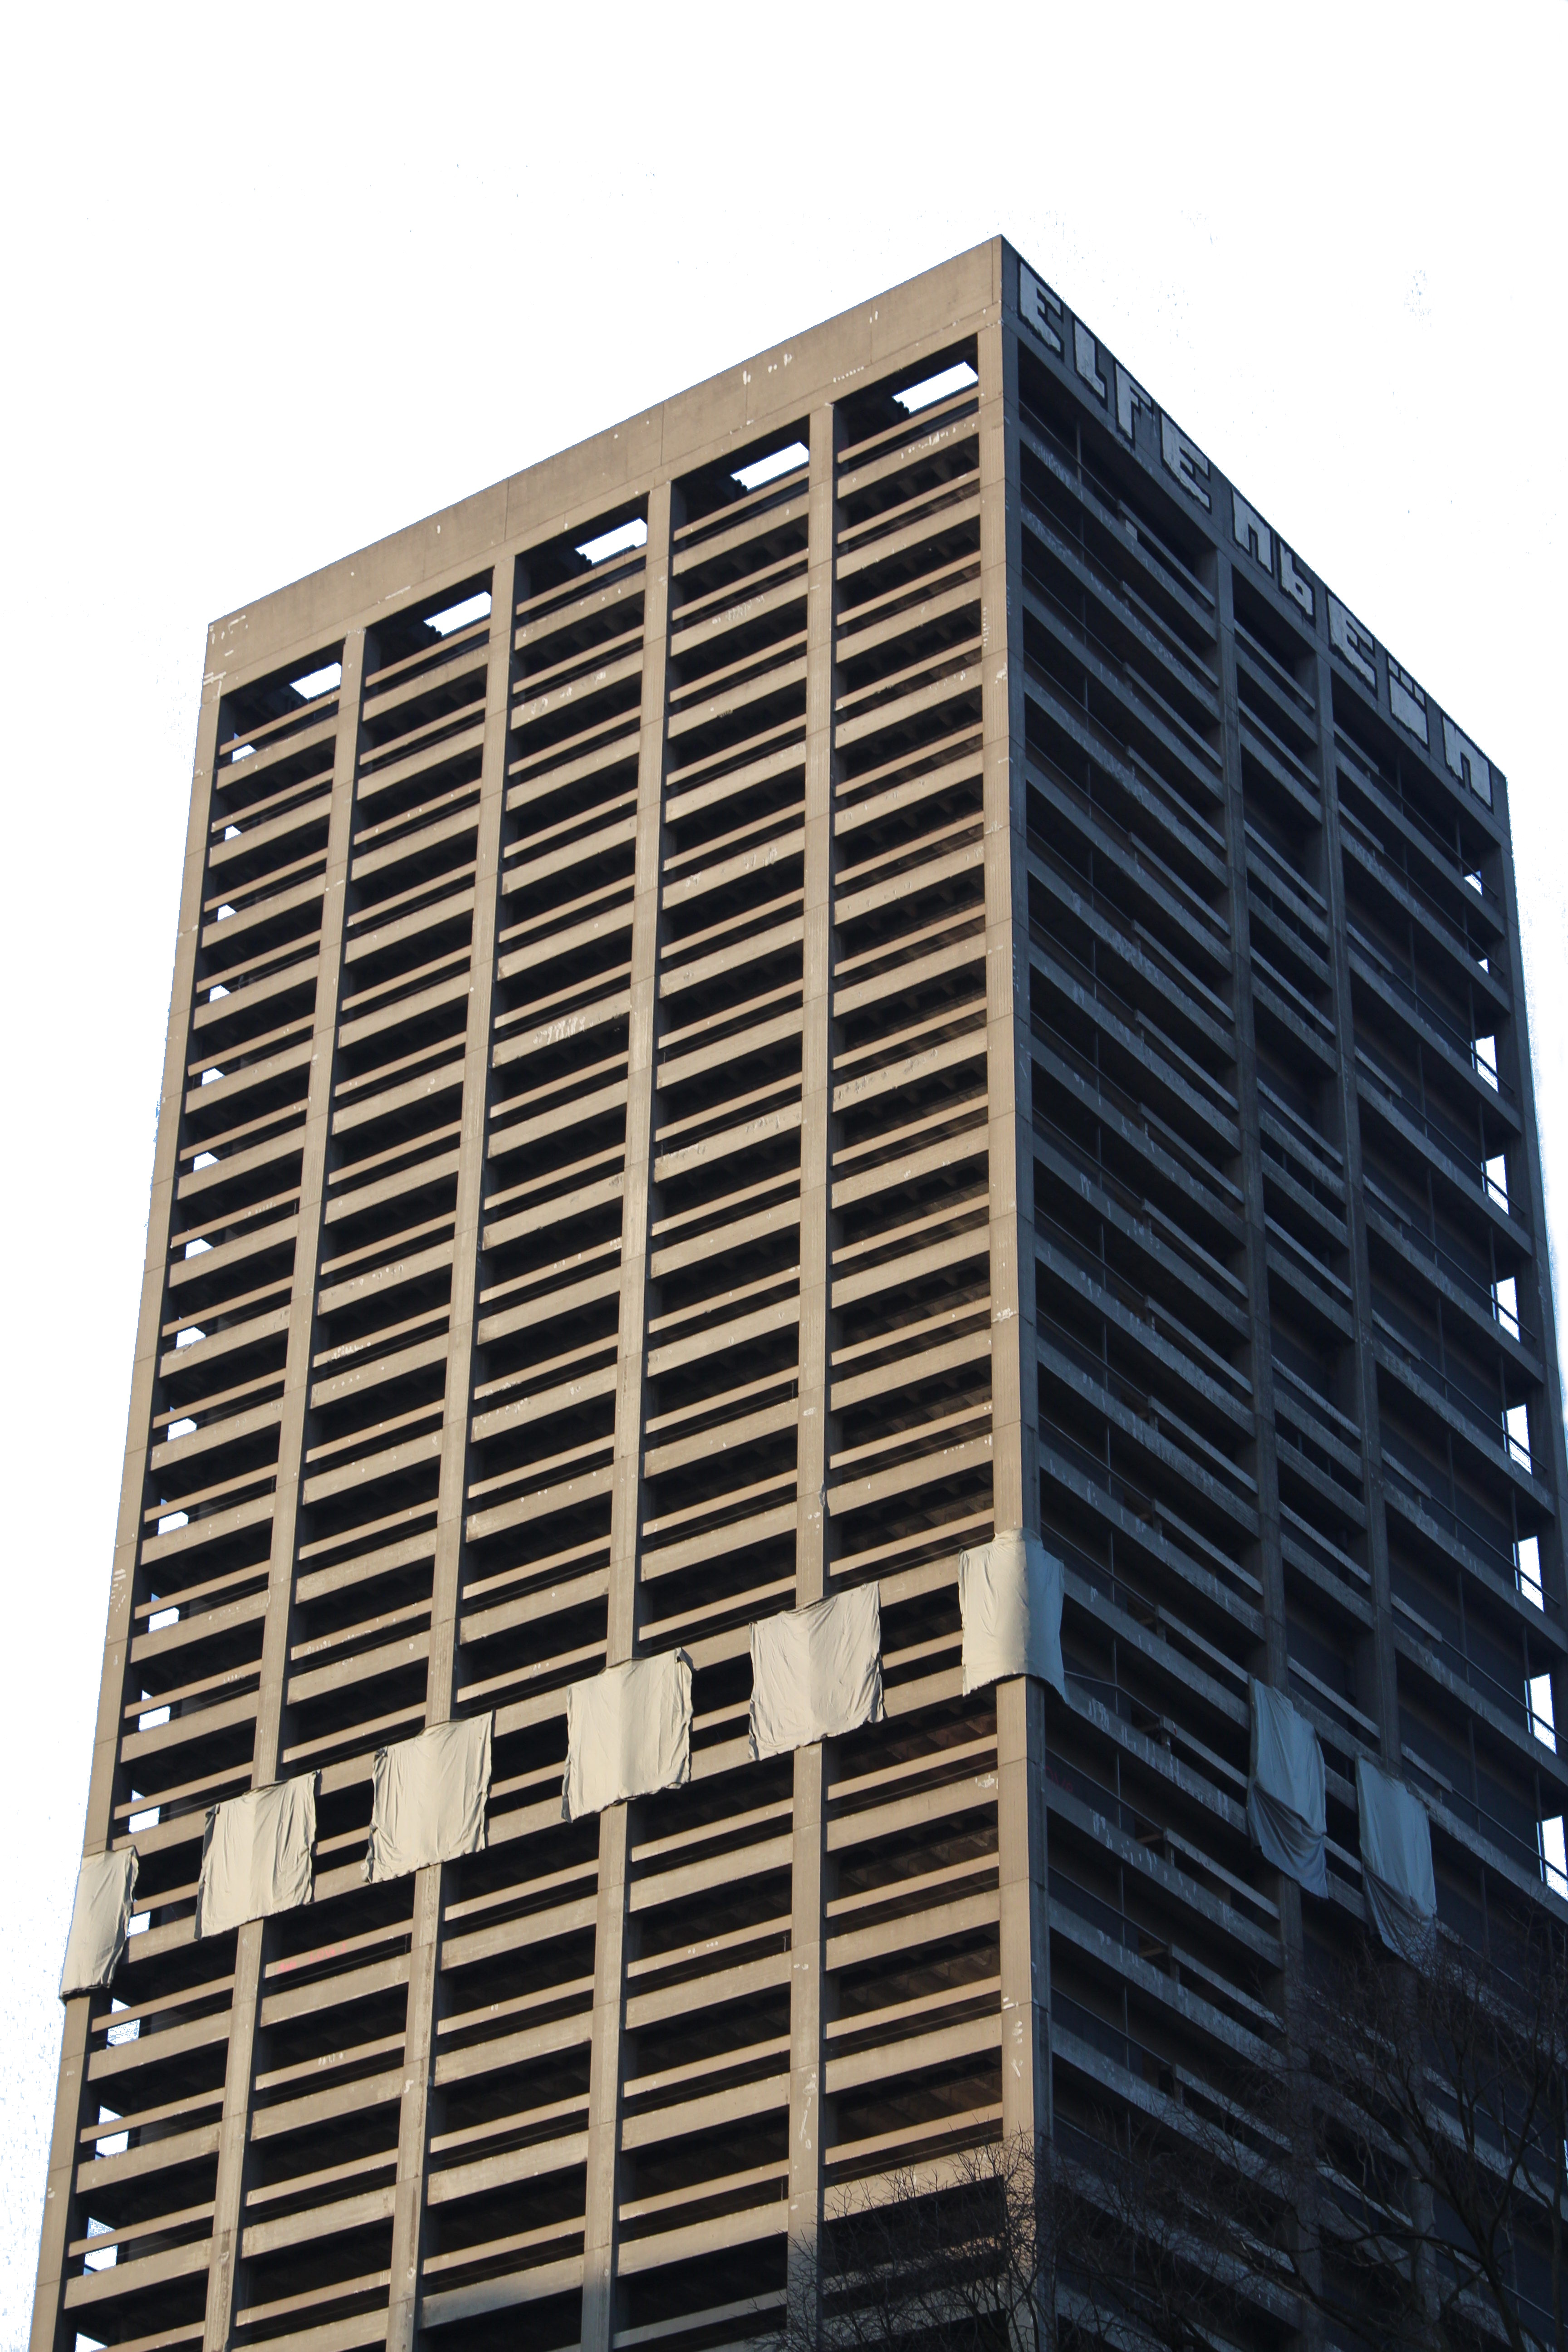
\includegraphics[width=0.28\textheight]{gfx/afeturm.jpg}
\caption[AfE-Turm]{AfE-Turm}
\label{gr:afeturm}
\end{figure}
\FloatBarrier

Zun\"achst beginnt eine \"ubersicht der verwendeten MVE-Software (Multi-View Environment) als auch der aktuellen Verfahren zur Registrierung von Bilddatens\"atzen. Anschlie\ss end erfolgt ein L\"osungsansatz zur interaktiven Aufteilung von Bildinhalten, welcher den sp\"ateren Rekonstruktionsansatz beschleunigen und dessen Qualit\"at maximieren soll. Dazu gliedert sich das Vorgehen wie folgt:
\newline
\newline
Kapitel 2 besch\"aftigt sich einf\"uhrend mit Grundlagen der verwendeten Programme und deren Verfahren um Bilddatens\"atze geometrisch zu registrieren.
\newline
\newline
Kapitel 3 beschreibt das aktuelle Verfahren zum Erstellen einer 3D-Rekonstruktion und dessen Probleme, dessen Einschr\"ankungen und den in diesem Projekt verfolgten L\"osungansatz.
\newline
\newline
Kapitel 4 behandelt die Merkmalsextraktion (engl.: Feature Extraction) der Fotografien mittels Regionsabgrenzungen als auch dessen Einfluss auf die verwendeten Algorithmen der Software. 
\newline
\newline
Kapitel 5 zeigt schlie\ss lich die Auswertung der Arbeit als auch eine Beurteilung der Rekonstruktionsergebnisse unter Ber\"ucksichtigung eines weiteren Datensatzes. Dabei liegt der Fokus auf der Qualit\"at und der Richtigkeit der Rekonstruktion.
\newline
\newline
Im Anschluss der vorgestellten Arbeit folgt ein Benutzerhandbuch in Bezug auf die resultierende Implementierung.

\chapter{Das verwendete Framework}
Zur Umsetzung der Aufgabe muss zun\"achst die Funktionsweise des aktuell verwendeten Verfahrens zur Auswertung und Rekonstruktion eines Bilddatensatzes analysiert werden. Dadurch soll eine Struktur f\"ur die anstehende Implementierung festgelegt werden, die in den existierenden Programmcode nur minimal eingreift. So muss der Code dahingehend modifiziert werden, dass die normale Funktionsweise nicht beeintr\"achtigt wird und das Programm bei Bedarf auch ohne die geplante Erweiterung funktionsf\"ahig bleibt.


\section{Multi-View Environment}
Das Multi-View Environment (MVE)\cite{fuhrmann2014mve} dient zur geometrische Oberfl\"achenrekonstruktion aus zuvor erfassten Bilddaten. Es implementiert eine end-to-end Pipeline dessen einzelne Abschnitte individuell ansprechbar sind. Fundament f\"ur jede Anwendung ist ein Datensatz an Fotografien eines Objektes, welche aus ausreichend vielen Winkeln akquiriert sein m\"ussen, damit eine l\"uckenlose 3D-Rekonstruktion erfolgen kann. Im ersten Abschnitt Structure-from-Motion (SfM) werden Bilder zu einander registriert indem jedes Foto eine Merkmalsextraktion durchl\"auft, die anschlie\ss end dazu dienen die eigentlichen Kamerapositionen zur\"uckzurechnen. Bilder werden samt ihrer detektierten Merkmale (engl.: Features) und anderer Parameter als Views zusammengefasst. Daraufhin ist es mittels Triangulation m\"oglich, \"uber korrespondierende Bildbereiche auf Tiefenwerte zu schlie\ss en und zweidimensionale Bildpunkte (x,y) in ein dreidimensionales Koordinatensystem (x,y,z) zu \"ubertragen, was den Vorgang des Multi-View Stereo (MVS) Abschnitts beschreibt. Als letztes erfolgt die Oberfl\"achentexturierung, die sich aus den Eingabebildern ergibt.

\subsection{Qt und die Benutzeroberfl\"ache}
Die einzelnen Schritte der MVE-Pipeline sind via Kommandozeile zug\"anglich, sodass zur leichteren Zug\"anglichkeit f\"ur Nutzer eine hauseigene, auf der Qt\footnote{\url{http://qt-project.org}} Bibliothek basierende Anwendung \glqq Ultimate MVE\grqq \ (UMVE) entworfen wurde. Jene soll in dieser Arbeit als Grundlage genutzt und um Funktionalit\"aten erweitert werden.\\
Die plattform\"ubergreifende C++ Klassenbibliothek Qt 4.0 bietet, anstelle des zuvor simuliertem Aussehens verschiedener Plattformen, native Schnittstellen an, um betriebssystemeigene Routinen zum Zeichnen der Oberfl\"achenelemente zu nutzen. Somit soll im Sinne der Aufgabenstellung eine Nutzerschnittstelle entworfen werden, die es erm\"oglicht einzelne Bildmerkmale mit inhaltlichem Bildkontext in Relation zu setzen. Die M\"oglichkeit Fotografien vorab manuell zu unterteilen erscheint notwendig um eine Relation zwischen Bildpunkten und ihrer zugeh\"origen Geb\"audeseite zu erstellen. Eine Anforderungsanalyse an die Nutzerschnittstelle ergibt ein Minimum an Funktionalit\"aten, die durch die Implementierung gew\"ahrleistet sein m\"ussen - die M\"oglichkeit Bildbereiche zu markieren, zu editieren und f\"ur das weitere Vorgehen verf\"ugbar zu machen. 


\subsection{Plugin-Integration}

Die zuvor genannte Qt Bibliothek soll verwendet werden um f\"ur die bereits bestehende Software eine Erweiterung zu implementieren. Die M\"oglichkeit die zugrundeliegende Software um Funktionalit\"aten zu erweitern, ist im Vergleich zu einem individuellen Programm vorteilhafter. Durch Implementierung einer externen Software entst\"unde die Notwendigkeit des Ein- und Auslesens notwendiger Daten. Damit die in MVE verwendeten Views nicht importiert und Ergebnisse des sp\"ater genauer beschriebenen Verfahrens nicht exportiert werden m\"ussen soll dieser Schritt in die MVE Pipeline integriert werden. Daher wurde sich auf eine modale Umsetzung in Form eines Plugins geeinigt, welches sich sp\"ater leicht in UMVE integrieren lassen soll. Zu den bereits bestehenden Darstellungen von UMVE kommt ein zus\"atzlicher Reiter hinzu, der trotz der Eingliederung die neuen Funktionalit\"aten getrennt anzeigt. Der Aufbau des geplanten Plugins orientiert sich dabei an bereits existierenden Ansichten der Software, sodass f\"ur den Nutzer eine gewohnte Arbeitsumgebung erhalten bleibt. 
\chapter{Problembeschreibung}
Die Problembehandlung beschreibt in diesem Abschnitt einen Ansatz, die anfangs fehlgeschlagene Rekonstruktion des AfE-Turms durch Typisierung der Bildmerkmale zu optimieren. 

\section{Aktueller Matchingansatz}
Rekonstruktionsmethoden werden als bildgebende Verfahren bezeichnet, deren Ziel eine dreidimensionale Ansicht des zu untersuchenden Objektes ist. Damit dies fehlerfrei geschieht, ist sowohl ein ausreichender Datensatz, als auch eine erfolgreiche vorangegangene Bildregistrierung notwendig. Das Matching ist Teil von SfM der MVE Pipeline und umfasst die Merkmalserfassung (engl.: Feature detection) innerhalb der Eingabedaten und die, auf Affinit\"aten beruhende Paarfindung (engl.: Feature matching). Dabei wird f\"ur jedes Bild eine Menge an Features erfasst (engl.: Featureset), die mit anderen verglichen werden. W\"ahrend jeweils immer ein Bilderpaar ausgewertet wird, werden mittels geeigneter Metrik die Merkmale des ersten auf die bestm\"oglich passenden des zweiten Bildes abgebildet und analog in die R\"uckrichtung. Das Ergebnis ist eine Menge an korrespondierenden Bildpunkten. Wenn zwei Features, die den gleichen Kontext beschreiben, auf einander abgebildet werden ist dies ein gefundener Match und kann dazu verwendet werden, die Parameter der einzelnen Kamerapositionen zu bestimmen. 
Liegen jene extrinsischen (i.d.R. Lage und Orientierung) und intrinsischen Kameraparameter (Parameter in Bezug auf die Kameralinse - radiale Verzerrung und Brennweite) vor, k\"onnen die beiden anderen Abschnitte der Pipeline folgen um Tiefenwerte und Texturierung zu bestimmen.

\section{Einschr\"ankungen und Problematik}
Wie bereits angesprochen zeigt die MVE Anwendung Defizite bei der Rekonstruktion von Modellen mit sich wiederholenden Texturen oder Oberfl\"achenstrukturen. Es l\"asst sich aktuell beobachten, dass f\"ur ein Featureset mit einer gro\ss en Anzahl an Elementen, die einen sehr \"ahnlichen Bildkontext beschreiben, oftmals Matches aufgenommen werden, die eigentlich nicht korrespondieren. In Bezug auf die Behandlung des AfE-Turms bedeutet das, es werden Bereiche der einen Fassade auf Bereiche der anderen projiziert. Die geometrische Relation der einzelnen Geb\"audeseiten ist nicht mehr gegeben und das Ergebnis ist eine sowohl verschobene als auch verzerrte Nachbildung des Turms.

\begin{figure}[h]
\centering
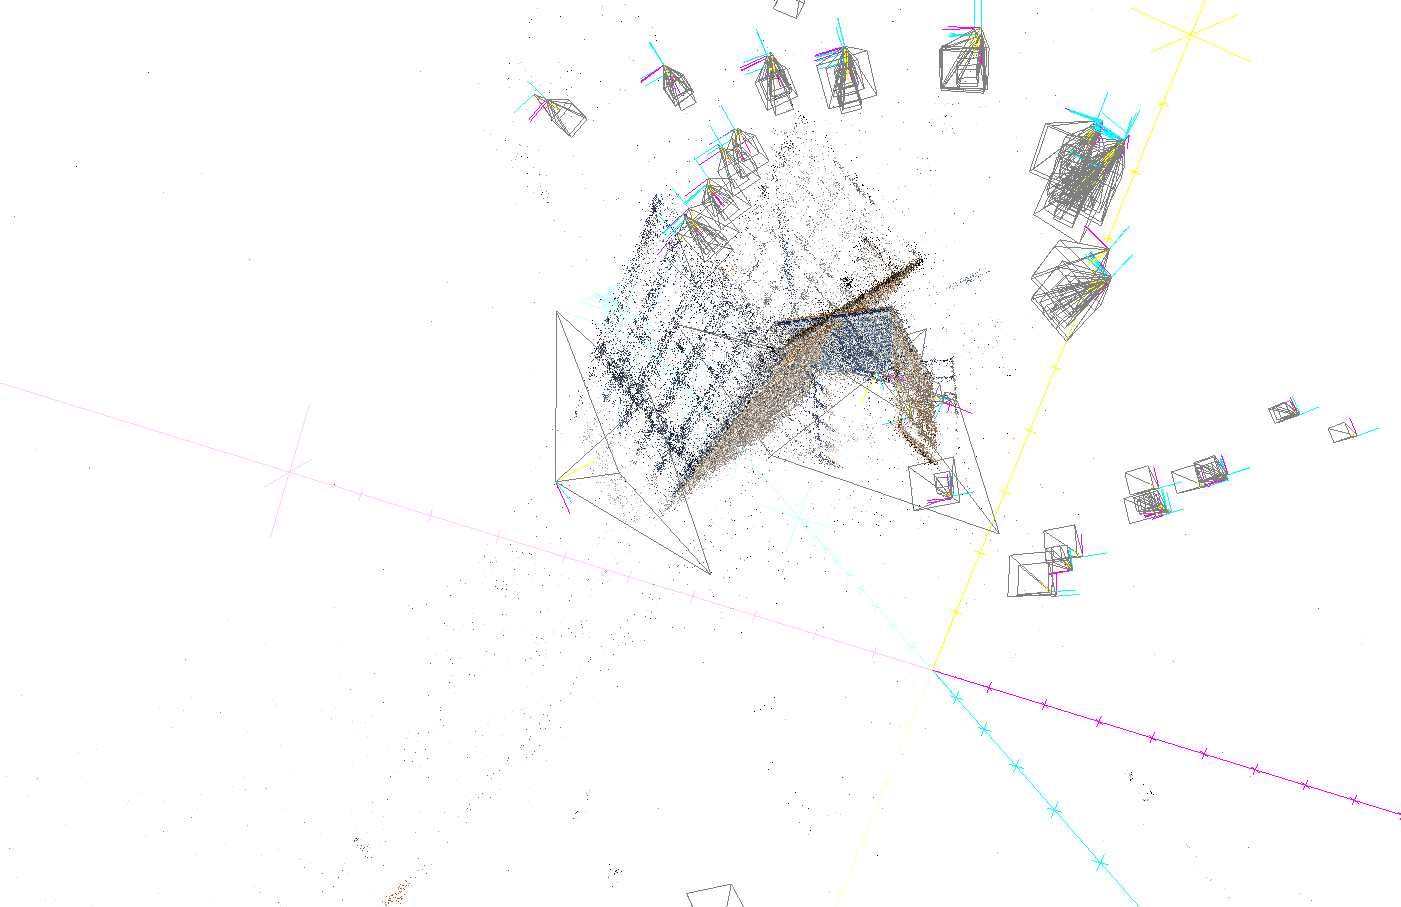
\includegraphics[height=0.3\textheight]{gfx/falscherekon1invert.png}
\caption[Fehlerhafte Rekonstruktion des AfE-Turms]{Fehlerhafte Rekonstruktion des AfE-Turms}
\label{gr:afeturmfehler}
\end{figure}
\FloatBarrier
Diese mangelhafte Rekonstruktion ist also auf eine fehlerhafte Paarbildung im Matchingverfahren zur\"uckzuf\"uhren, was gleichzeitig die Pr\"amisse des L\"osungsansatzes ist. 

\section{L\"osungsansatz und geplantes Vorgehen}
Da das Matchingverfahren im Moment f\"ur den Datensatz des AfE-Turms fehlschl\"agt, muss dieser Abschnitt der Software angepasst werden. Der hier vorgestellte Ansatz umfasst folglich die schon zuvor erw\"ahnten Anpassungen.\\
Durch die zus\"atzlichen Informationen die jedem Feature angeh\"oren, wird bei der Projektion eines Featuresets auf ein anderes die Definitionsmenge eingeschr\"ankt. Zu jedem Feature l\"asst sich \"uberpr\"ufen, welcher Region es angeh\"ort. Wohingegen zuvor nur eine Metrik als \"ahnlichkeitsma\ss  verwendet wurde, wird nun zuvor \"uberpr\"uft, ob ein korrespondierendes Feature-Paar auch den gleichen Regionen angeh\"ort, d.h. so k\"onnen keine fehlerhaften Feature-Paare mehr entstehen, dessen Elemente unterschiedlichen Regionen zugeteilt sind. Zwar nimmt mittels manueller Aufteilung der Fotografien das Verfahren vorab eine gewisse Zeit in Anspruch, die sich jedoch sp\"ater durch die gefilterte und somit reduzierte Feature-Menge in einem schnelleren und vor allem qualitativ besseren Rekonstruktionsablauf \"au\ss ern sollte.

\subsection{Bedeutung der Regionsabgrenzung}
Die MVE Pipeline besteht wie in den vorangegangenen Kapiteln beschrieben aus drei einzelnen Schritten, n\"amlich SfM, MVS und der Texturierung. Da sich SfM mit der Kalkulation der extrinsischen und intrinsischen Kameraparameter befasst und dazu die Regionierungsparameter bereits vorliegen m\"ussen, ist das Verfahren eindeutig davor einzuordnen. 

\begin{figure}[h]
\centering
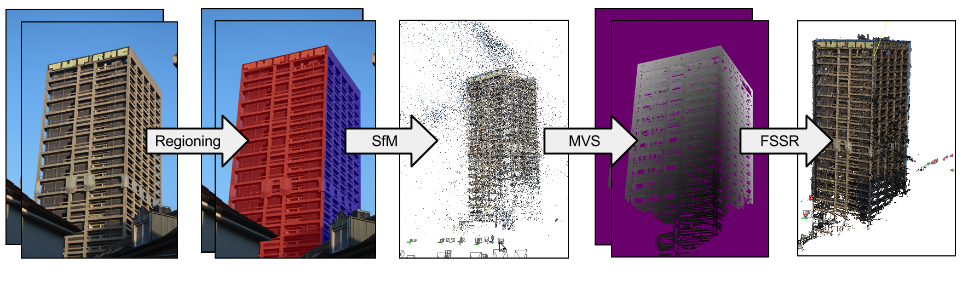
\includegraphics[width=0.9\textwidth]{gfx/pipeline.png}
\caption[MVE Pipeline]{MVE Pipeline}
\label{gr:pipeline}
\end{figure}
\FloatBarrier
\chapter{Regionenbasiertes Matching}
Die vorab beschriebenen Parameter der Bildaufteilung flie\ss en nun in den Matchingprozess mit ein und sollen dazu verwendet werden, fehlerhafte Matches zu filtern.

%CITE

\section{Regionierung des Datensatzes}
Ein Begriff der die Isolation eines Bereiches innerhalb eines Bildes beschreibt und eng mit der Bedeutung der Segmentierung und Klassifikation zusammenh\"angt. Dabei werden hier, anhand von Vorwissen, Bildregionen mit zus\"atzlichen Informationen bez\"uglich ihrer geometrischen Lage versehen. Das Unterteilen eines Bildes in verschiedene Bereiche impliziert zun\"achst die Funktionalit\"at eine Region zu definieren, die eine Teilmenge aller Bildpunkte enth\"alt. \"Uber diese Masken l\"asst sich im Folgenden leicht bestimmen, ob sich ein Bildpunkt innerhalb oder au\ss erhalb dieser befindet. Die Form einer Region wird dabei \"uber die manuell gesetzten Eckpunkte und der dadurch eingeschlossenen Fl\"ache festgelegt.\\
Als angepasster Ansatz wurde sich f\"ur eine polygone Regionsabgrenzung der unterschiedlichen Fassaden entschieden, wobei theoretisch Vierecke gen\"ugen w\"urden. Jedoch lassen sich durch eine polygone Fl\"ache m\"uhelos Verdeckungen, wie andere Bauwerke oder Vegetation, innerhalb der Fotos umgehen, die jene Au\ss enseiten des AfE-Turms bedecken.

\begin{figure}[h]
\centering
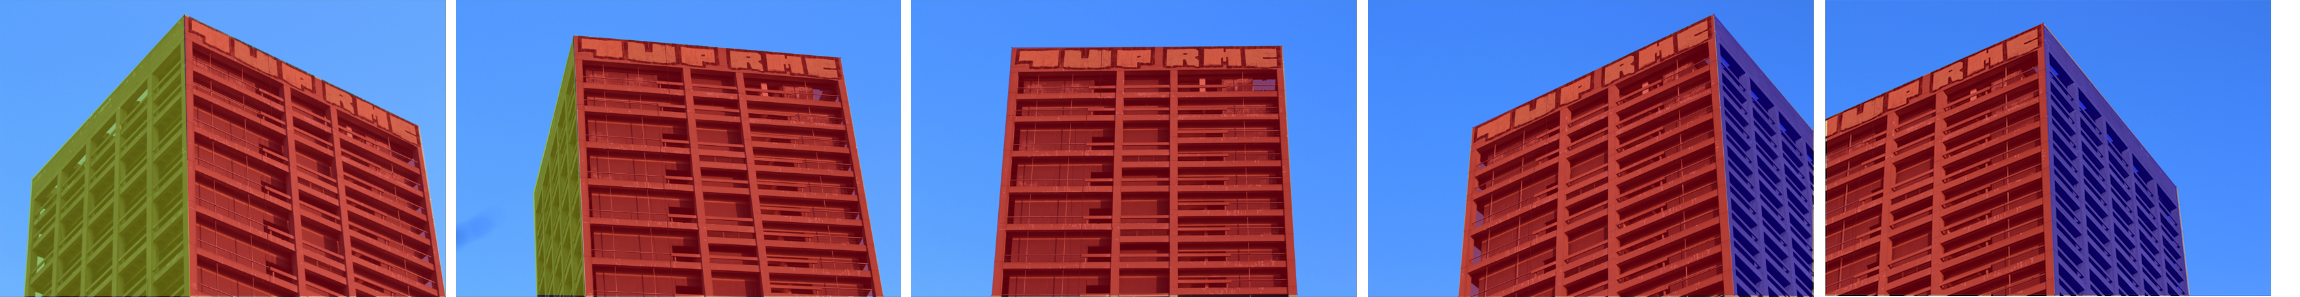
\includegraphics[width=0.9\textwidth]{gfx/regreihe.png}
\caption[F\"unf regionierte Bilder des AfE-Turms]{F\"unf regionierte Bilder des AfE-Turms}
\label{gr:afeturmreg}
\end{figure}
\FloatBarrier

Wichtig ist zu erw\"ahnen, dass nicht nur vorab festgelegte Regionen eines Bildes vom angepassten Matchingverfahren ber\"ucksichtigt werden, sondern auch noch immer Features aus nicht markierten Bereichen betrachtet werden. So hat jeder unterteilte Bereich eine eindeutige Identifikation, ebenso wie nicht markierte. Alle au\ss erhalb der Regionen liegende Bildpunkte werden zu einer \glqq Unknown\grqq \ Region (Regions-ID: -1) zusammengefasst. Dieser Bereich wird also wie eine Region behandelt und dessen Features werden nur mit anderen Features gematcht, die auch in dieser \glqq Unknown\grqq \ Region liegen.\\
Dieser Ansatz soll fehlerhafte Matches entfernen, jedoch zutreffende unber\"uhrt lassen.

\subsection{Schnitttest einer Region}
Um zu \"uberpr\"ufen, ob bestimmte Bildpunkte einer gewissen Region angeh\"oren, ist es f\"ur das sp\"atere Matchingverfahren n\"otig, dass vor dem Matching \"uberpr\"uft werden kann, ob ein vermeintbares Feature-Paar auch zul\"assig ist. Hierzu wird mittels Strahl-Methode des Punkt-in-Polygon-Tests nach Jordan\cite{hake1994kartographie}\cite{bartelme1995geoinformatik} \"uberpr\"uft, ob sich ein Bildpunkt innerhalb einer der Regionen befindet. Ein Polygon l\"asst sich auch als eine Menge gerichteter Liniensegmente betrachten. Bei der Strahl-Methode wird, vereinfacht gesagt, vom zu testenden Punkt aus ein Strahl in eine beliebige Richtung gesendet und die Anzahl der Schnittpunkte mit den Liniensegmente gez\"ahlt. Bei ungerader Zahl befindet sich der Punkt innerhalb des Polygons und andersherum bei gerader Anzahl au\ss erhalb. Ein gro\ss er Vorteil dieser Methode ist, dass sowohl konvexe als auch konkave Polygone gleicherma\ss en behandelt werden k\"onnen. 

\section{Das RGN-Dateiformat}
Zus\"atzlich zu den einzelnen Views, deren zugeh\"orige Parameter in einer MVE-Datei abgelegt sind, m\"ussen somit auch Informationen zu Form und Position der zugeh\"origen Regionen aufgenommen werden. Im Sinne der Wiederverwendbarkeit, wird hierf\"ur ein eigenes Dateiformat 
definiert anstatt die Regionsparameter in bereits existierende Softwareigene Dateitypen zu schreiben. Somit l\"asst sich auf jene Parameter zugreifen, auch ohne einen kompletten View zu laden.\\
Regionen werden pro View in eine RGN-Datei geschrieben. Das hier verwendete Format enth\"alt sowohl relative Positionen der Eckpunkte aller Polygone als auch deren Identifizierung und setzt sich wie folgt zusammen:


\begin{table}[h]
\begin{tabular}{|c|}
\hline
\begin{tabular}[c]{@{}c@{}}Region 1-ID\\ x-Koordinate Punkt 1\\ y-Koordinate Punkt 1\\ ...\\ x-Koordinate Punkt n\\ y-Koordinate Punkt n\end{tabular} \\ \hline
\begin{tabular}[c]{@{}c@{}}Region 2-ID\\ x-Koordinate Punkt 1\\ y-Koordinate Punkt 1\\ ...\\ x-Koordinate Punkt n\\ y-Koordinate Punkt n\end{tabular} \\ \hline
...                                                                                                                                                   \\ \hline
\begin{tabular}[c]{@{}c@{}}Region n-ID\\ x-Koordinate Punkt 1\\ y-Koordinate Punkt 1\\ ...\\ x-Koordinate Punkt n\\ y-Koordinate Punkt n\end{tabular} \\ \hline
\end{tabular}
\caption[Aufbau des RGN-Dateiformats]{Aufbau des RGN-Dateiformats}
\label{tab:rgn}
\end{table}

Falls f\"ur einen Datensatz an Fotografien f\"ur jedes Bild eine Regionierung vorgenommen wurde, existieren folglich ebenso viele RGN-Dateien wie MVE-Dateien.

\section{Matchingansatz}
Rekonstruktionen mittels Bilddaten, die ein sehr homogenes und gleichm\"a\ss ig texturiertes Modell zeigen, k\"onnen oftmals fehlschlagen, da bei der Merkmalsextraktion Korrespondenzen in Bildern erfasst werden, die tats\"achlich nicht zugeh\"orig sind.\\
Durch die Regionierung liegen nun zus\"atzliche Informationen vor mit denen \"uberpr\"uft wird, ob zwei zu testende Feature-Punkte zul\"assig sind. Genauer bedeutet das, es wird mit der zuvor beschriebenen Strahl-Methode f\"ur jedes Feature \"uberpr\"uft, ob und welcher der Regionen es zugeh\"orig ist. Somit k\"onnen vorm eigentlichen Matchingansatz schon unzutreffende Korrespondenzen ausgeschlossen werden, indem nur Elemente aus Regionen mit selber ID verglichen werden. Damit kein m\"oglicher Match ausgeschlossen wird, werden auch die nicht markierten Bildbereiche ber\"ucksichtigt und untereinander gematcht.
\chapter{Evaluation}
Um die Rekonstruktionsqualit\"at der Ergebnisse auswerten zu k\"onnen folgt der Vergleich einer normalen MVE Rekonstruktion zu jener verbesserten Variante des Frankfurter AfE-Turms. Zur Evaluation der Resultate dieser Arbeit werden zwei unterschiedliche Datens\"atze verwendet um die Robustheit der algorithmischen Optimierungen zu zeigen, wobei eines den genannten Turm und das andere den Triumphbogen (Arc de Triumphe) in Paris zeigt. Dazu wird zuerst \\
Die Umsetzung des L\"osungsansatzes wurde mittels C++ gel\"ost und aufbauend auf dem MVE Framework und der Qt Bibliothek wurden diese implementiert.

\section{Genauigkeit der Regionsabgrenzung}
Damit auf die Zugeh\"origkeit der einzelnen Bildpunkte zu ihren jeweiligen Geb\"audefassaden geschlossen werden kann, m\"ussen sich diese innerhalb einer der festgelegten Bereiche befinden. Dabei ist ein Simplex die kleinstm\"ogliche Form einer Region, d.h. ein n-dimensionales Polytop\footnote{Polytop beschreibt ein Polygon beliebiger Dimension} mit n+1 Eckpunkten. In dem Fall m\"ussen mindestens drei Eckpunkte pro Region gegeben sein um in der zweidimensionalen Ebene eine Fl\"ache zu definieren. Dahingegen ist die Anzahl der Eckpunkte nach oben hin unbeschr\"ankt. \\
Das Regionierungsverfahren ist in der Lage sowohl konvexe als auch konkave Polygone zu behandeln. Sind Regionen an ihren Kanten zu umgebenden Bildbereichen visuell unterscheidbar und dessen Bildelemente zugeh\"orig identifizierbar, gen\"ugt zur Umrandung einer Region auch lediglich eine konvexe H\"ulle aller relevanten Bildpunkte. Die detailgenaue Segmentierung konkaver Polygone ist meist nur innerhalb homogener Bildbereiche n\"otig. 

\begin{figure}[h]
\centering
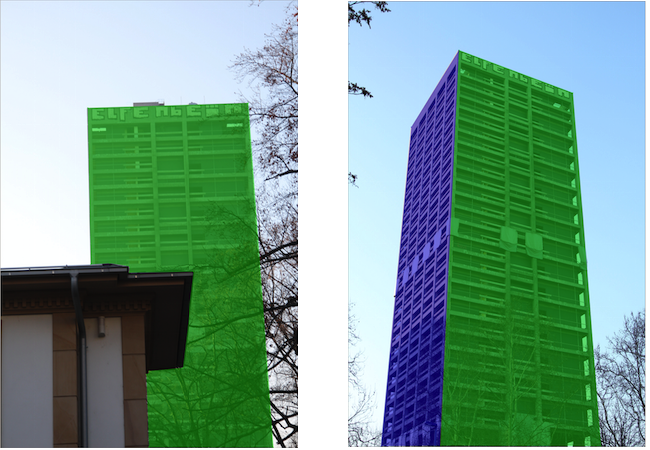
\includegraphics[width=0.9\textwidth]{gfx/konvexkonkav.png}
\caption[Links: Konkave Regionierung Rechts: Konvexe Regionierung]{Links: Konkave Regionierung Rechts: Konvexe Regionierung}
\label{gr:konreg}
\end{figure}
\FloatBarrier

\section{Auswertung regionierter Rekonstruktionen}

In diesem Abschnittl werden die Ergebnisse und Einfl\"usse der Regionierung  auf eine Rekonstruktion zweier Datens\"atze (AfE-Turm in Abschnitt 5.5.1 und der Triumpfbogen, Paris in Abschnitt 5.5.2) vorgestellt und mit den Ergebnissen ohne eine vorherige Regionierung verglichen.

\subsection{AfE-Turm}
Zu Beginn dieses Projektes existierte eine fehlerhafte Rekonstruktion, mit unzureichender Bildqualit\"at. Die Darstellung der unzureichenden Rekonstruktion, die Ausgangspunkt dieses Projektes war, wurde bereits in den vorherigen Kapiteln gezeigt, jedoch in texturierter Form.

\begin{figure}[h]
\centering
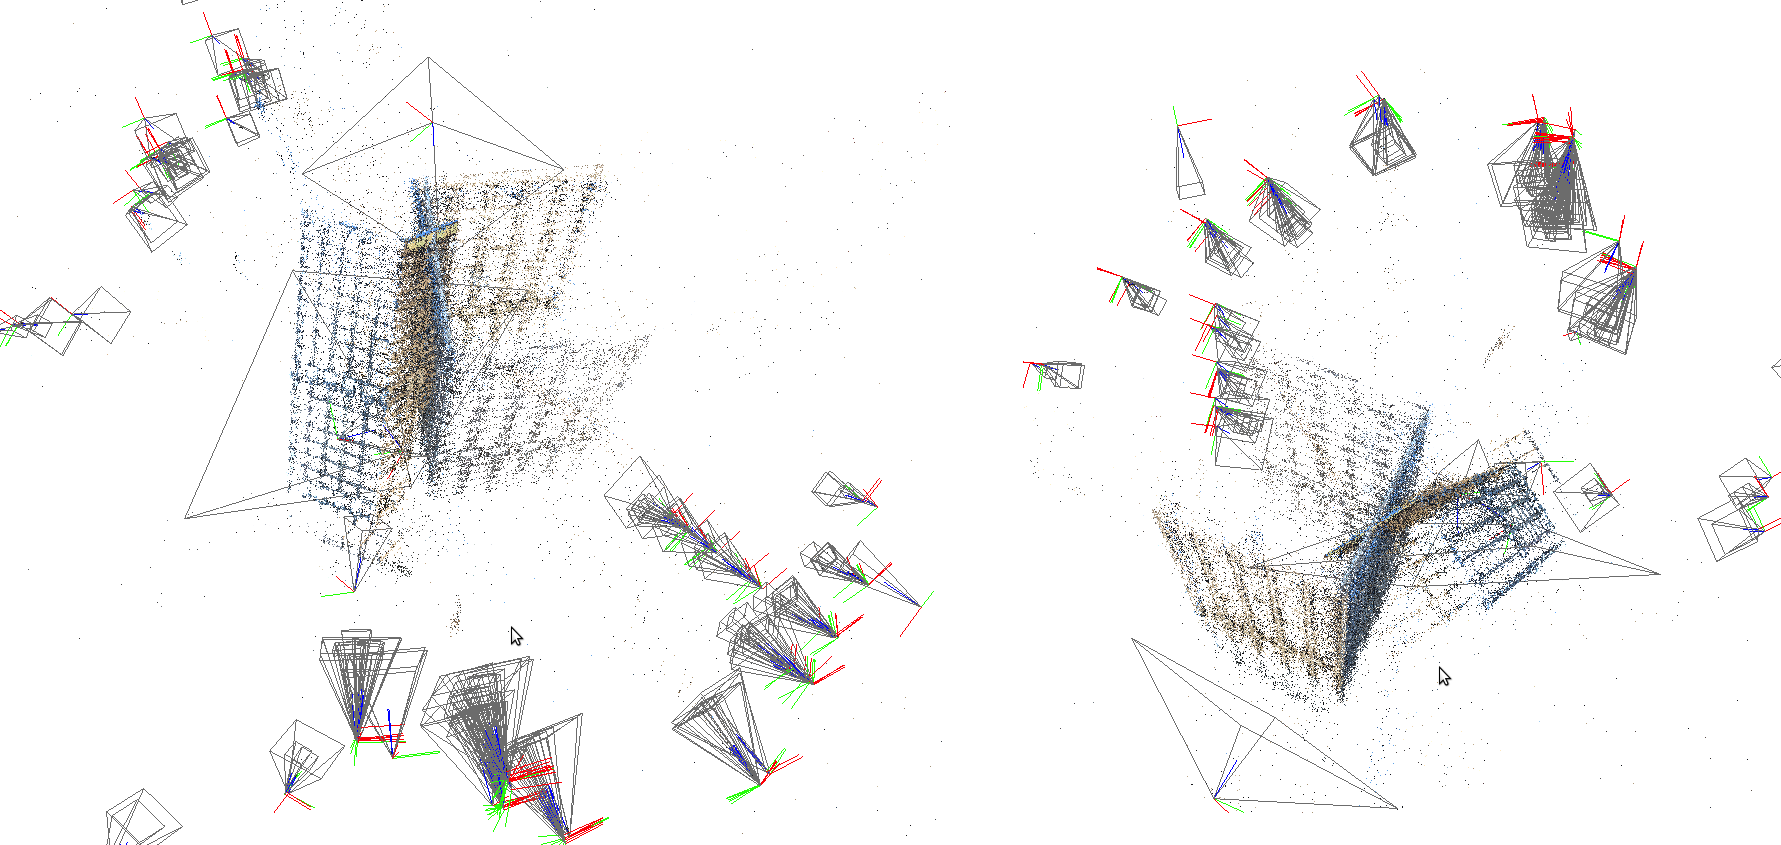
\includegraphics[width=0.9\textwidth]{gfx/Evaluation/prePointcloud_AfEboth.png}
\caption[Punktwolken Drauf- und Seitenansicht der mangelhaften Rekonstruktion]{Punktwolken Drauf- und Seitenansicht der mangelhaften Rekonstruktion}
\label{gr:seitefehler}
\end{figure}
\FloatBarrier

Der anf\"angliche Matchingansatz wurde erweitert, sodass dieser weitere Parameter bez\"uglich der Regionierung ber\"ucksichtigt und das vorher auftretende Artefaktverhalten reduziert. Die Qualit\"at dieses Verfahrens soll hier im Folgenden beurteilt werden. Dazu dienen reale Messdaten des behandelten Frankfurter AfE-Turms, sowie ein Datensatz des Arc de Triomphe in Paris. Als Vergleich der Qualit\"at werden Rekonstruktionen mit und ohne diese erweiterte Methode herangezogen. \\
Stellt man die Ergebnisse eines unbehandelten mit denen eines regionierten Datensatzes gegen\"uber, lassen sich deutliche Unterschiede erkennen. Im ersten Ansatz wird die Rekonstruktion auf geometrische Korrektheit der einzelnen Fassaden \"uberpr\"uft, wobei Positionierung und Orientierung der Geb\"audeseiten f\"ur ein brauchbares Ergebnis stimmen m\"ussen. 

\begin{figure}[h]
\centering
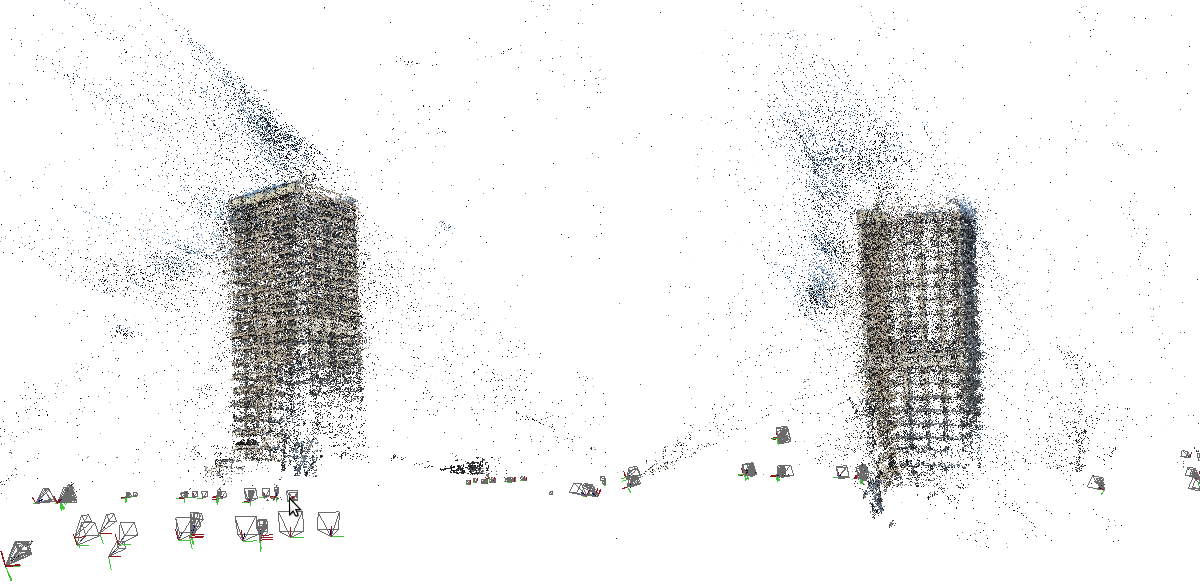
\includegraphics[width=0.9\textwidth]{gfx/Evaluation/finalPointcloud_AfE.png}
\caption[Die Seitenansicht einer Rekonstruktion eines zuvor regionierten Datensatzes]{Die Seitenansicht einer Rekonstruktion eines zuvor regionierten Datensatzes}
\label{gr:seitereg}
\end{figure}
\FloatBarrier

\begin{figure}[h]
\centering
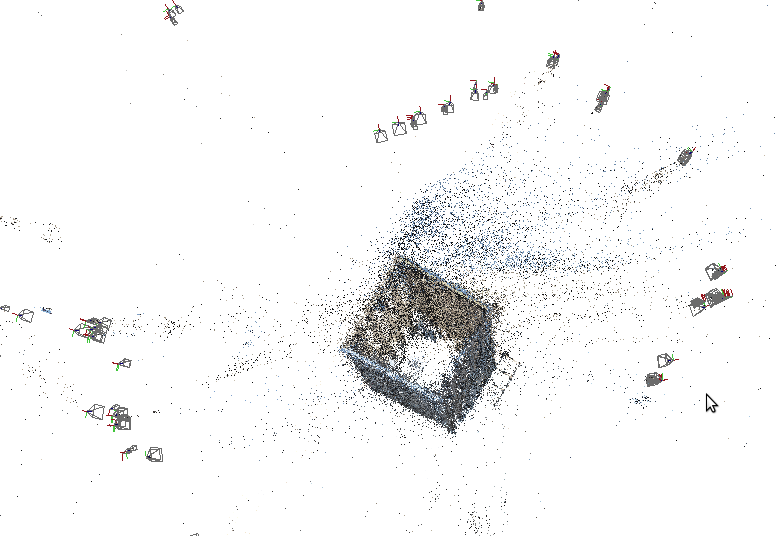
\includegraphics[width=0.9\textwidth]{gfx/Evaluation/finalPointcloud_Top_AfE.png}
\caption[Die Draufsicht einer Rekonstruktion eines zuvor regionierten Datensatzes]{Die Draufsicht einer Rekonstruktion eines zuvor regionierten Datensatzes}
\label{gr:draufreg}
\end{figure}
\FloatBarrier

Neben der nun geometrisch korrekten Ausrichtung der einzelnen Fassaden, bezeugt auch die Anordnung der einzelnen Kameras ein sinnvolles Resultat. Durch das Regioning-Plugin ist UMVE in der Lage vorher falsche Kameraparameter zu korrigieren und die Szene fehlerfrei darzustellen.\\
Insgesamt hat das gezeigte Verfahren Rekonstruktionsfehler entfernt und mehr 3D-Punkte an korrekten Stellen produziert. Hinzu kamen lediglich einige Abbildungen des Himmels, die durch Verdeckungen vereinzelter B\"aume entstanden.

\begin{figure}[h]
\centering
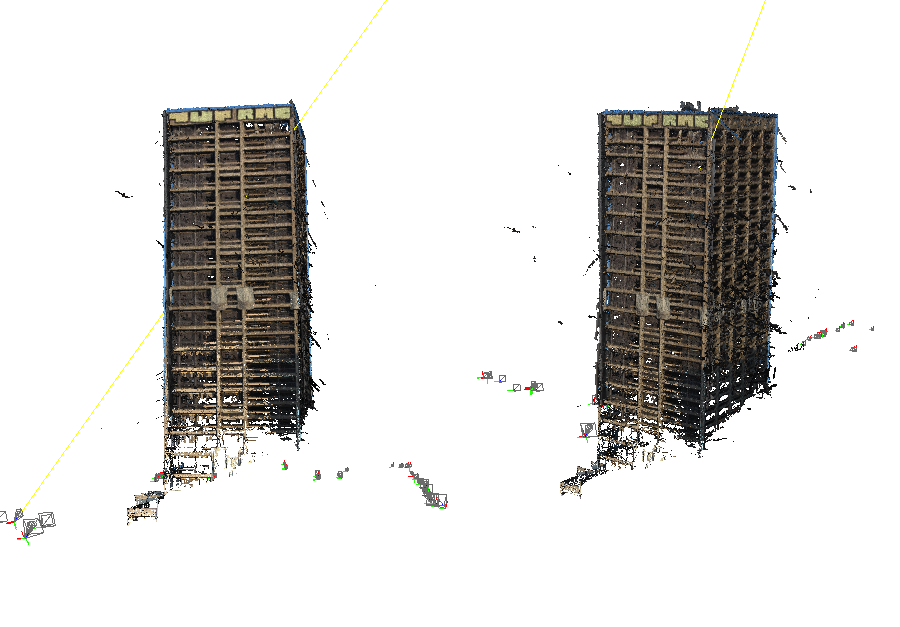
\includegraphics[width=0.9\textwidth]{gfx/Evaluation/finalReconstruction_AfE.png}
\caption[Zwei Seitenansichten einer fehlerfreien Rekonstruktion mit Hilfe des Regioning-Plugins]{Zwei Seitenansichten einer fehlerfreien Rekonstruktion mit Hilfe des Regioning-Plugins}
\label{gr:seitezwei}
\end{figure}
\FloatBarrier

\subsection{Arc de Triomphe}

Als zweiter Datensatz wurde der Arc de Triomphe, Paris gew\"ahlt. Dessen Vorder- und R\"uckseite sind schwierig zu unterscheiden, wodurch sich vermuten l\"asst, dass hier eine Regionierung zu einem besseren Ergebnis f\"uhrt.\\
Tats\"achlich ist es so, dass der Algorithmus bei einer Rekonstruktion ohne Regionierung die Vorder- und R\"uckseite des Triumpfbogens nicht unterscheiden kann und zwischen diesen Matches findet (siehe Abbildung \ref{gr:matchohne}).\\
Durch die Regionierung der Bilddaten und den Ausschluss unzul\"assiger Korrespondenzen ist folglich die Anzahl der detektierten Matches verh\"altnism\"a\ss ig geringer, da fehlerhafte als auch region\"ubergreifende aussortiert wurden. Die folgenden Abbildungen veranschaulichen die Auswirkung regionierter Eingabedaten und unbehandelter in Bezug auf die erfassten Matches.

\begin{figure}[h]
\centering
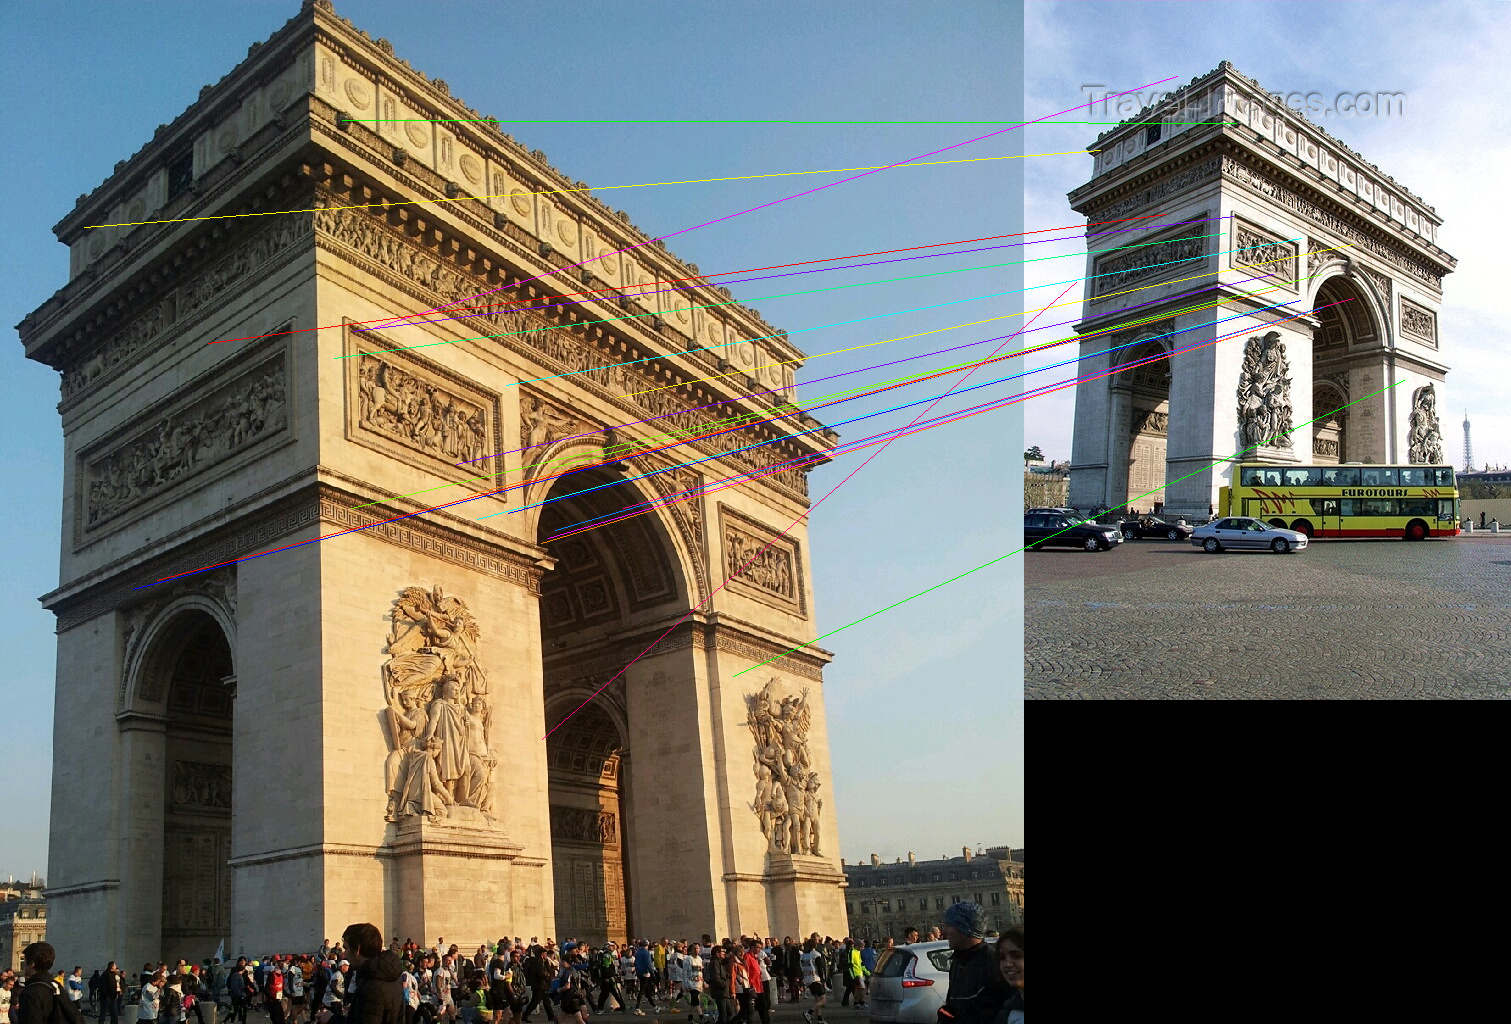
\includegraphics[width=0.9\textwidth]{gfx/Matchingpaare/matching_109_107.png}
\caption[Gefundene Matches zweier unterschiedlicher Seiten ohne Regionierung]{Gefundene Matches zweier unterschiedlicher Seiten ohne Regionierung}
\label{gr:matchohne}
\end{figure}
\FloatBarrier

\begin{figure}[h]
\centering
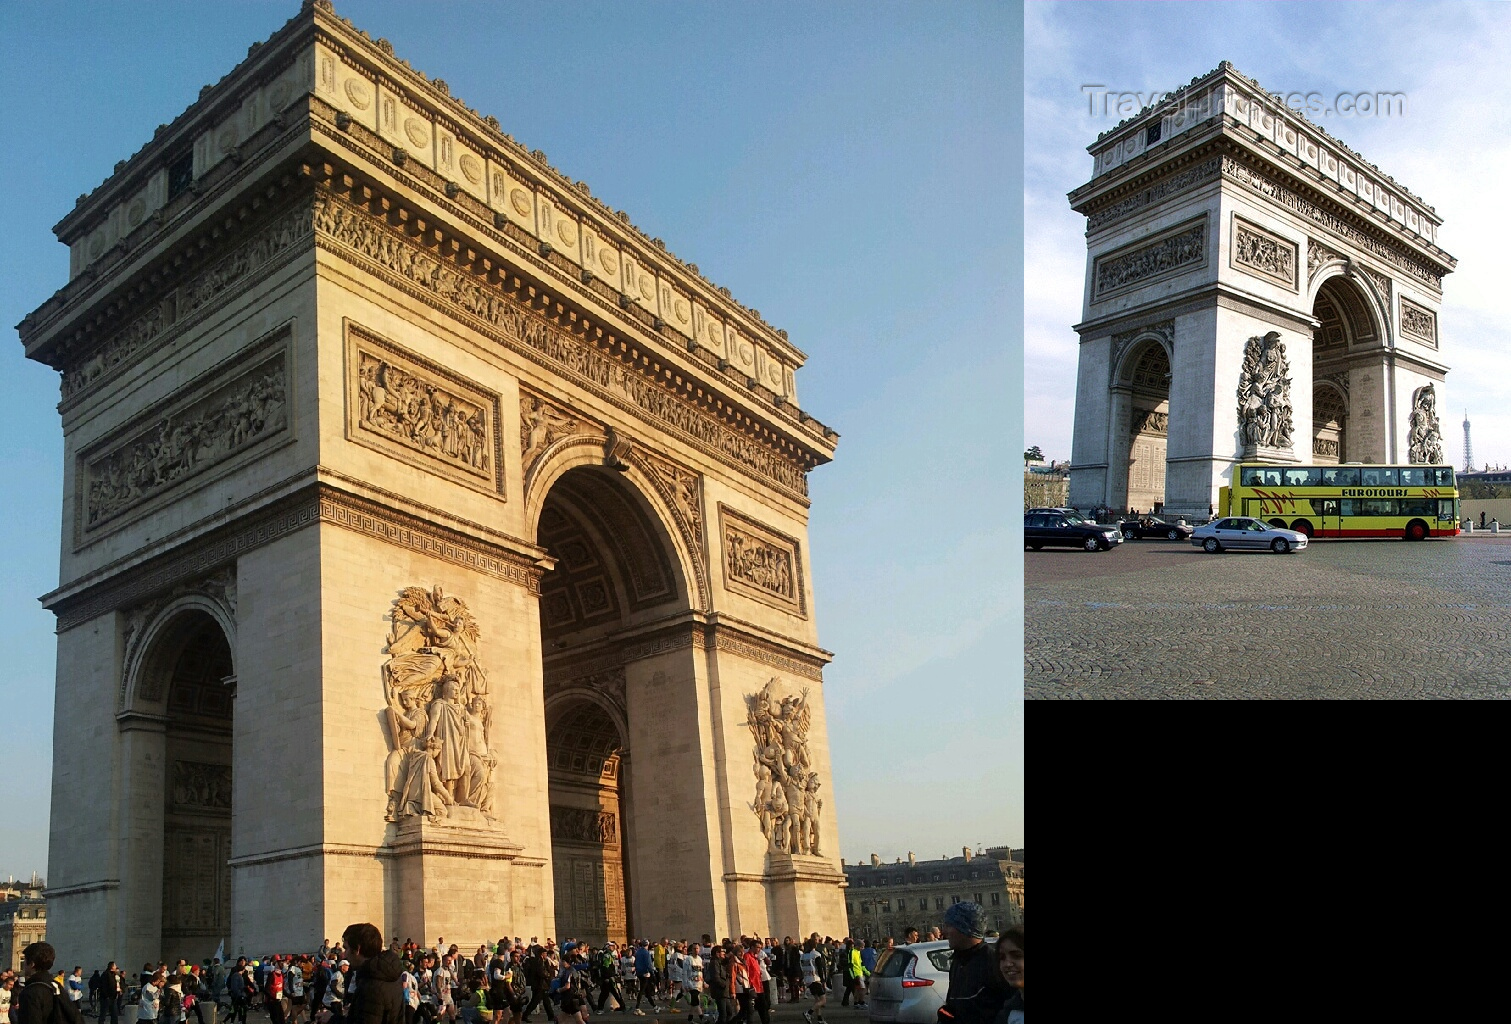
\includegraphics[width=0.9\textwidth]{gfx/Matchingpaare/region_109_107.png}
\caption[Gefundene Matches zweier unterschiedlicher Seiten mit Regionierung]{Gefundene Matches zweier unterschiedlicher Seiten mit Regionierung}
\label{gr:matchmit}
\end{figure}
\FloatBarrier

Dadurch ist eine Unterscheidung zwischen Vorder- und R\"uckseite m\"oglich. Die folgenden Bilder zeigen einen Vergleich zwischen einer Rekonstruktion des Triumpfbogens ohne eine Regionierung (Abbildung \ref{gr:arcohne}) und mit einer Regionierung (Abbildung \ref{gr:arcmit}).

\begin{figure}[h]
\centering
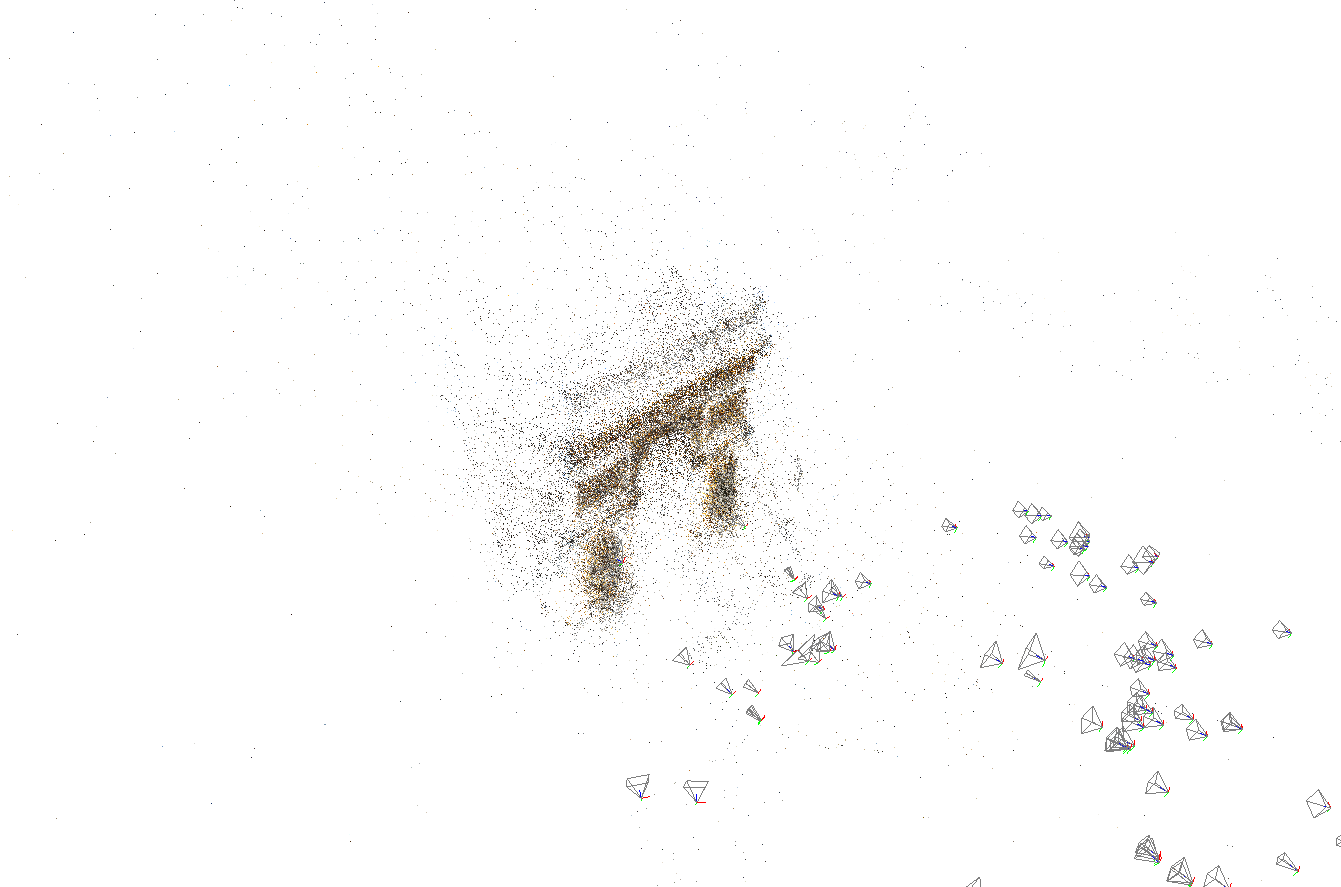
\includegraphics[height=0.34\textheight]{gfx/arcohne.png}
\caption[Rekonstruktion des Triumpfbogens ohne Regionierung]{Rekonstruktion des Triumpfbogens ohne Regionierung}
\label{gr:arcohne}
\end{figure}
\FloatBarrier

\begin{figure}[h]
\centering
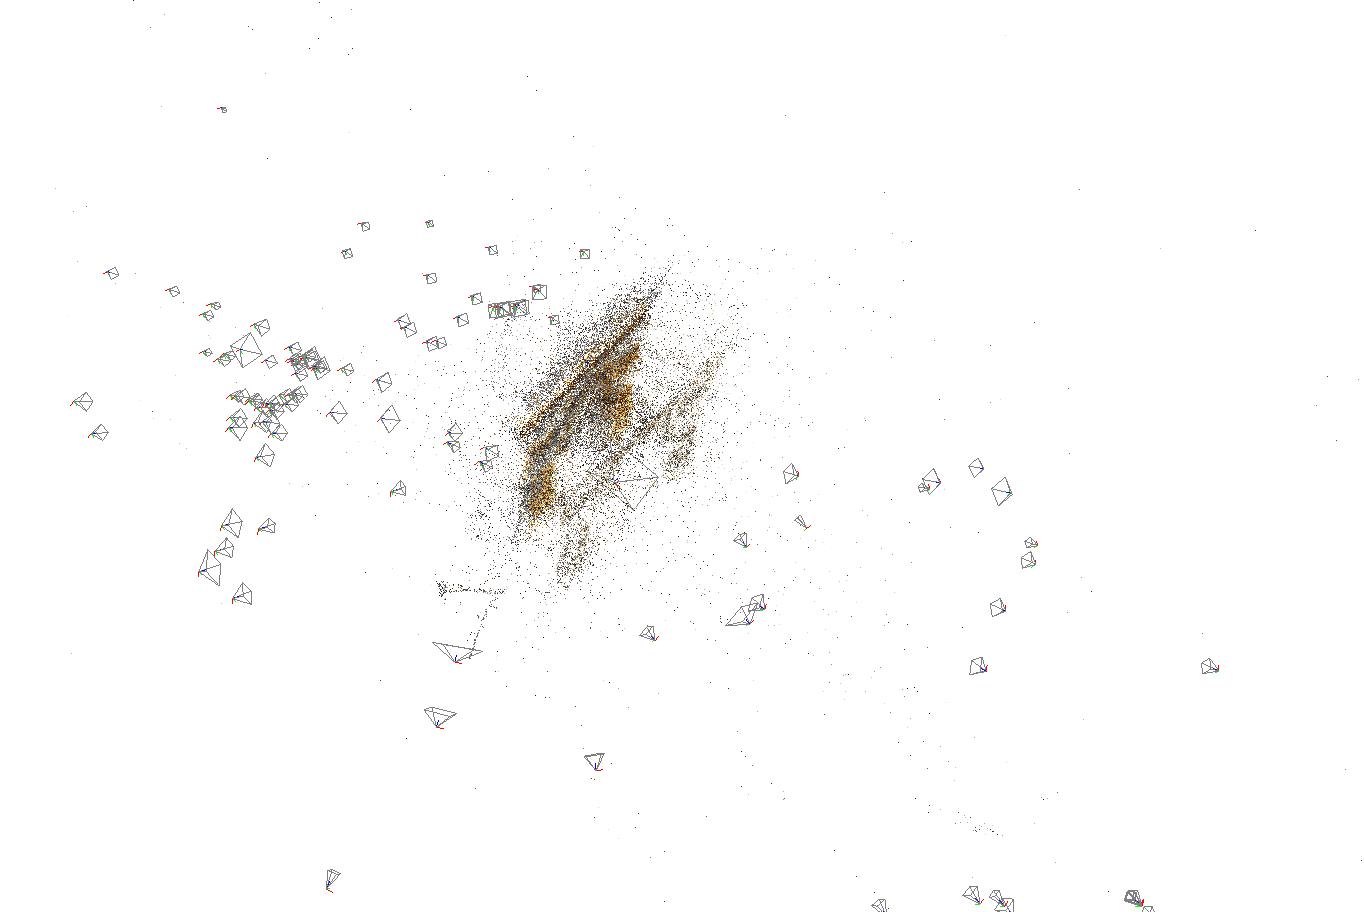
\includegraphics[height=0.34\textheight]{gfx/arcmit.png}
\caption[Rekonstruktion des Triumpfbogens mit Regionierung]{Rekonstruktion des Triumpfbogens mit Regionierung}
\label{gr:arcmit}
\end{figure}
\FloatBarrier

\section{Performanz}
Ohne eine Unterteilung der Eingabebilder in Regionen vergleicht UMVE jedes Feature des ersten Views mit jedem Feature des zweiten Views, was einer quadratischen Laufzeit entspricht. Wurden die Eingabebilder in Regionen unterteilt, werden Features, die in Regionen unterschiedlicher IDs liegen, vom Matchingalgorithmus ausgeschlossen. Da der Matchingalgorithmus bei entsprechend vielen Features eine zeitkritische Komponente der Laufzeit ist, kann so eine Performanzsteigerung durch die Regionierung der Daten resultieren.\\
Die im Folgenden beschriebene Durchf\"uhrung bezieht sich auf den Datensatz des AfE-Turms dessen Eingabebilder jeweils in der Breite und H\"ohe halbiert wurden. Der f\"ur die Ausf\"uhrung verwendete Computer (Intel\textsuperscript{\textregistered} Xeon\textsuperscript{\textregistered} Processor E3-1231 v3
(8M Cache, 3.40 GHz)) erzielte f\"ur eine normale Rekonstruktion mit unbehandeltem Datensatz eine Laufzeit von 50 Minuten. Wohingegen die Durchf\"uhrung mit regionierten Bilddaten eine Dauer von 12 Minuten ergab. Das zeigt eine Verbesserung der Performanz ungef\"ahr um den Faktor 4. F\"ur den Datensatz mit Bildern (verschiedene Aufl\"osungen) des Triumphbogens ergeben sich Laufzeiten von 23 Minuten ohne und 5 Minuten mit Regionierung, was einer Verbesserung der Performanz um den Faktor ca. 4,5 entspricht.
\chapter{Benutzerhandbuch}
Dieses Handbuch bezieht sich auf das UMVE Regioning-Plugin Version 1.0. Es enth\"alt detaillierte Anleitungen zum Ausf\"uhren bestimmter Funktionen mit diesem Plugin.

\section{\"Ubersicht}

\begin{figure}[h]
\centering
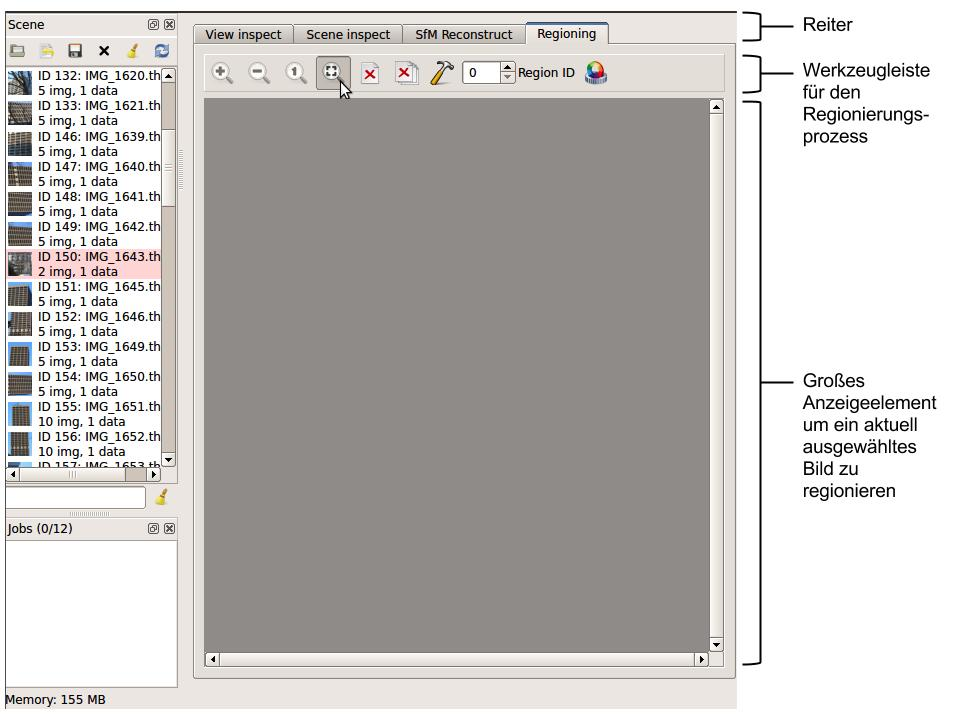
\includegraphics[width=0.9\textwidth]{gfx/Handbuch/RegioningPluginOverview.jpg}
\caption[\"Ubersicht \"uber das UI des Plugins]{\"Ubersicht \"uber das UI des Plugins}
\label{gr:uebersicht}
\end{figure}
\FloatBarrier

Das Plugin erscheint als zus\"atzlicher Reiter neben den bereits bestehenden (View inspect, Scene inspect, SfM Reconstruct) am oberen Rand des UMVE Fensters. Die Darstellung teilt sich hierbei einerseits in die Leiste mit den unterschiedlichen Werkzeugen und andererseits in die Anzeige der Bilddaten.

\section{Die Bildanzeige}
Das Plugin l\"asst sich \"uber die gewohnte Datenauswahl in der Scene am linken Rand steuern, sodass ein Klick auf das gew\"unschte Thumbnail gen\"ugt und das ausgew\"ahlte Bild erscheint in dem Anzeigeelement. Die Bildanzeige wird jeweils im Bearbeitungsmodus als auch im Regionierungsmodus verwendet und auch wie die Darstellung des aktuellen Bildes l\"asst sich dies \"uber die dar\"uber liegende Werkzeugleiste steuern (Hierzu mehr im folgenden Kapitel).

\newpage

\section{Werkzeuge und Arbeitsschritte}

\begin{figure}[h]
\centering

\includegraphics{gfx/Handbuch/toolbar.png}
\caption[Werkzeugleiste des Plugins]{Werkzeugleiste des Plugins}
\label{gr:toolbar}
\end{figure}
\FloatBarrier

Um die verschiedenen Werkzeuge zu verwenden, muss vorerst ein beliebiger Bilddatensatz ge\"offnet werden. Dabei werden unterschiedliche M\"oglichkeiten der Bilddarstellung und der Bearbeitung gezeigt.\\
Folgende Funktionalit\"aten stehen nun zur Verf\"ugung:\\
\begin{itemize}
\item \textbf{Vergr\"o\ss erungs- und Verkleinerungsfunktionen}

\begin{figure}[h]
\centering

\includegraphics{gfx/Handbuch/zoom.png}
\caption[Zoom-Funktionen des Plugins]{Zoom-Funktionen des Plugins}
\label{gr:zoom}
\end{figure}
\FloatBarrier

Mittels dieser Funktionen l\"asst sich, f\"ur eine genauere Regionsabgrenzung die Gr\"o\ss enansicht des Bildes regulieren. So sind die ersten beiden Symbole zur inkrementellen Vergr\"o\ss erung (einzoomen) als auch zur Verkleinerung (auszoomen). Eine verkleinerte Darstellung des Bildes ist n\"utzlich um einen \"Uberblick der bisherigen Regionierung zu sehen. Das dritte Lupensymbol, durch die \glqq 1\grqq \ gekennzeichnet, setzt den vorherigen Zoomfaktor wieder zur\"uck und zeigt das Bild in Originalgr\"o\ss e. Im Gegensatz dazu passt das vierte Symbol die Darstellung auf die Bildschirm- bzw. Fenstergr\"o\ss e an.
\newline
\item \textbf{Regionen entfernen}

\begin{figure}[h]
\centering

\includegraphics{gfx/Handbuch/delete.png}
\caption[L\"oschen-Funktionen des Plugins]{L\"oschen-Funktionen des Plugins}
\label{gr:loeschen}
\end{figure}
\FloatBarrier

Um bereits gezeichnete oder bearbeitete Regionen wieder zu l\"oschen gibt es diese beiden Funktionen. \"Uber die Region-ID Auswahl l\"asst sich eine zu l\"oschende ID ausw\"ahlen und durch das erste Symbol diese dann entfernen. Das zweite Symbol hingegen l\"oscht alle bestehenden Regionen aus dem aktuell ausgew\"ahlten Bild.
\newline
\newpage
\item \textbf{Regionierungs- und Bearbeitungsmodus}

\begin{figure}[h]
\centering
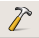
\includegraphics{gfx/Handbuch/edit.png}
\caption[Symbol zum \"Andern des Modus]{Symbol zum \"Andern des Modus}
\label{gr:modus}
\end{figure}
\FloatBarrier

Das Symbol ist zu Beginn nicht ausgew\"ahlt, was bedeutet, dass sich das Plugin im Regionierungsmodus befindet. \"Uber die linke Maustaste lassen sich nun beliebig viele Punkte setzen um eine Region abzugrenzen und mit der rechten Maustaste l\"asst sich schlie\ss lich das Polygon schlie\ss en. Vorrausetzung f\"ur diese Aktion ist, dass mindestens drei Punkte gesetzt wurden, die dann eine Fl\"ache aufspannen. Dazu wird der zuletzt gezeichnete Punkt mit dem ersten verbunden. Dabei spielt es keine Rolle, ob die Polygone konkav oder konvex gezeichnet sind. Wird eine zweite Region mit bereits existierender ID neu gezeichnet, so wird die erste entfernt und ersetzt. \\
Ist dieses Hammersymbol ausgew\"ahlt befindet sich das Plugin im Bearbeitungsmodus. \"Uber die Region-ID l\"asst sich hierf\"ur die zu bearbeitende Region ausw\"ahlen. Um die Form eines Polygons zu ver\"andern wird mit der linken Maustaste an die Stelle im Bild geklickt, zu der sich die bestehende Region ausdehnen bzw. verringern soll. Da kein expliziter Eckpunkt bestimmt wird, der seine Position ver\"andern soll, wird der Punkt gew\"ahlt, der der neu bestimmten Position am n\"achsten ist.
\newline
\item \textbf{Regions-ID Auswahl}

\begin{figure}[h]
\centering
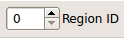
\includegraphics{gfx/Handbuch/regionID.png}
\caption[Regions-ID Auswahlfeld des Plugins]{Regions-ID Auswahlfeld des Plugins}
\label{gr:auswahl}
\end{figure}
\FloatBarrier

Diese Funktion wird nicht nur beim Zeichnen verwendet um der momentanen Region eine ID zuzuweisen, sondern auch bei den vorher beschriebenen Optionen. So muss die gew\"unschte ID gew\"ahlt werden, wenn eine bestimmte Region gel\"oscht oder bearbeitet werden soll. Wichtig ist, dass es maximal 8 verschiedene Regionen geben kann, wobei jede einzelne eine feste Farbzuweisung hat.
\newline
\item \textbf{Farbzuweisung der Regions-IDs}

\begin{figure}[h]
\centering
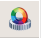
\includegraphics{gfx/Handbuch/chroma.png}
\caption[Farbzuweisungssymbol des Plugins]{Farbzuweisungssymbol des Plugins}
\label{gr:chroma}
\end{figure}
\FloatBarrier

Diese Funktion dient eigentlich nicht der Regionierung selbst, sondern \"offnet ein separates Fenster. Dieses zeigt eine Zuweisung der verwendeten Farben zu den zugeh\"origen IDs. Die Farbvergabe ist vorgegeben und beschr\"ankt die Anzahl verschiedener Regionen auf acht.

\begin{figure}[h]
\centering
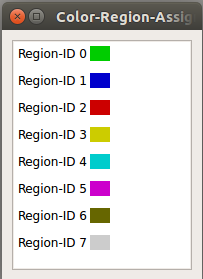
\includegraphics{gfx/cols.png}
\caption[Regions-ID-Farbzuweisung des Plugins]{Regions-ID-Farbzuweisung des Plugins}
\label{gr:zuweisung}
\end{figure}
\FloatBarrier

\end{itemize}

\section{Automatische Speicherfunktion}
F\"ur das anschlie\ss ende Matchingverfahren m\"ussen die Regionierungsparameter verf\"ugbar gemacht werden. Dazu m\"ussen gezeichnete Regionen in das vorgesehene Dateiformat geschrieben werden. Um Situationen zu vermeiden, in denen gezeichnete Regionen oder Ver\"anderungen vergessen werden zu speichern oder bei einem Bildwechsel verloren gehen, existiert eine automatische Speicherfunktion. Das automatische Speichern betrifft hierbei folgende Aktionen:\\
\begin{itemize}
\item Das Einzeichnen und Abschlie\ss en einzelner Regionen
\item Das Bearbeiten einzelner Regionen
\item Das L\"oschen einzelner oder aller Regionen
\end{itemize}
Jede einzelne Modifikation der Regionierungsparameter wird festgehalten, sodass eine manuelle Speicherung entf\"allt und man bedenkenlos nach Fertigstellung der Regionierung das n\"achste Bild \"offnen kann.

	
	%======================================================
	% The back matter
	%======================================================
	%\cleardoublepage
	\refstepcounter{dummy}
	\listoffigures
	\addcontentsline{toc}{chapter}{Abbildungsverzeichnis}
	\listoftables
	\addcontentsline{toc}{chapter}{Tabellenverzeichnis}
	\bibliographystyle{plainnat} % <--- layout of the bib
	\bibliography{bibliography} % file name of your bib
	\addcontentsline{toc}{chapter}{\bibname}


\end{document}
%======================================================
%======================================================